\chapter{Αξιολόγηση}

Για την αξιολόγηση του νέου συστήματος αρχείων στο \osv{}, διεξάγαμε δοκιμές
συγκρίνοντας με τα υπόλοιπα διαθέσιμα συστήματα αρχείων αλλά και το
\viofs{} στο \linux{}, όπου η σύγκριση είχε νόημα. Οι δοκιμές περιλαμβάνουν
τρία σενάρια, όπως αναλύονται στη συνέχεια: ένα συνθετικό μετροπρόγραμμα
(\en{synthetic benchmark} ή \en{microbenchmark}), μια δοκιμή χρόνου εκκίνησης
και τέλος μία πραγματική εφαρμογή (\en{application benchmark}).

\section{Μεθοδολογία}
Όλες οι δοκιμές πραγματοποιήθηκαν σε προσωπικό υπολογιστή με τα στοιχεία που
αναφέρονται στον πίνακα \ref{tab:host-specs}, ενώ ο πίνακας
\ref{tab:guest-specs} περιλαμβάνει τις προδιαγραφές των \osv{} και \linux{}
\en{guests}. Ως προς τη διεξαγωγή τους πρέπει να αναφερθούν τα εξής:
\begin{itemize}
    \item Για την εκτέλεση όλων των δοκιμών χρησιμοποιήθηκε ένα προσωρινό
          σύστημα αρχείων (\emph{\en{tmpfs}}) % ref https://www.kernel.org/doc/html/v5.8/filesystems/tmpfs.html
          στον \host{}, τόσο για τις εικόνες του \osv{} όσο και για τους
          κοινόχρηστους καταλόγους στην περίπτωση των \viofs{} και \en{NFS}.
          Αυτό έγινε ώστε να μην επηρεάζονται οι επιδόσεις από τη συσκευή
          αποθήκευσης του \host{}.
    \item Η δυναμική προσαρμογή της συχνότητας της \en{CPU} ήταν
          απενεργοποιημένη, χρησιμοποιώντας τον \emph{\en{``performance'' CPU
          scaling governor}} % ref https://www.kernel.org/doc/html/v5.8/admin-guide/pm/cpufreq.html
          στον \host{}.
    \item Η διεργασία του \qemu{} ήταν απομονωμένη από τις υπόλοιπες
          (\en{virtiofsd, perf, vegeta}) ως προς τις \en{CPUs} στις οποίες
          εκτελούνταν (\emph{\en{CPU pinning}}). % ref https://man7.org/linux/man-pages/man2/sched_setaffinity.2.html
          Συγκεκριμένα, στο \qemu{} αφιερώνονταν επεξεργαστικοί πυρήνες
          ισάριθμοι με το πλήθος των \en{CPUs} του \guest{}, ενώ οι υπόλοιπες
          προαναφερόμενες διεργασίες δεσμεύονταν στους υπόλοιπους διαθέσιμους.
          Αυτό έγινε με σκοπό την ελαχιστοποίηση των παρεμβολών που θα μπορούσαν
          να επηρεάσουν τις επιδόσεις.
    \item Για τη μέτρηση της χρησιμοποιούμενης επεξεργαστικής ισχύος (\en{CPU
          usage}) επελέγη το \emph{\en{perf}} \cite{perf}, στην έκδοση
          5.7.g3d77e6a8804a. Συγκεκριμένα, χρησιμοποιήθηκε η εντολή
          \texttt{\en{perf stat}}, με το \en{``task-clock'' perf event}. Η
          μέτρηση έγινε για τη διεργασία του \qemu{}, το \en{virtiofsd}, το
          \en{vhost kernel thread} και τα \en{NFS kernel threads} (για το καθένα
          όπου ήταν εφαρμόσιμο):
    \item Όλες οι δοκιμές επαναλήφθηκαν \emph{10 φορές}, από τις οποίες στη
          συνέχεια παρουσιάζονται η μέση τιμή \en{mean} και η τυπική απόκλιση
          \en{standard deviation}. Στην περίπτωση του \osv{} κάθε επανάληψη ήταν
          μία εκ νέου εκκίνηση της εικονικής μηχανής, ενώ στο \linux{} όλες οι
          επαναλήψεις έγιναν στην ίδια εκτέλεση της εικονικής μηχανής.
    \item Το \en{virtiofsd} εκτελούνταν με το \en{cache mode} απενεργοποιημένο
          (\texttt{\en{cache=none}}) και ένα \en{thread}
          (\texttt{\en{--thread-pool-size=1}}). Το δεύτερο επελέγη διότι
          οδηγούσε σε ελαφρώς πιο συνεπείς μετρήσεις, χωρίς όμως να παρατηρείται
          καλύτερη επίδοση όπως είχε αναφερθεί σε συζήτηση στη \en{mailing list}
          του \viofs{}%
          \footnote{\en{\url{https://www.redhat.com/archives/virtio-fs/2020-September/msg00068.html}}}.
    \item Για την εκτέλεση του \osv{} έγινε χρήση του βοηθητικού \en{script}
          (\en{scripts/run.py}) που παρέχει, το οποίο τροποποιήθηκε για την
          διεξαγωγή των δοκιμών, ώστε να ενορχηστρώνει την εκτέλεση όλων των
          υπόλοιπων εργαλείων (\en{virtiofsd, perf, vegeta}). Ως προς τη
          δικτύωση της εικονικής μηχανής, χρησιμοποιήθηκε το \emph{\en{tap
          backend}} % ref https://www.qemu.org/docs/master/system/invocation.html#hxtool-5
          του \qemu{} με το \emph{\en{vhost}} ενεργοποιημένο, ενώ στο \en{VM}
          δινόταν στατική διεύθυνση \en{IP}.
    \item Ως \en{NFS server} χρησιμοποιήθηκε η αντίστοιχη υλοποίηση του \linux{}
          στον \host{}. Όλες οι δοκιμές έγιναν με την έκδοση 3 του \en{NFS},
          καθώς η έκδοση 4 δεν ήταν λειτουργική από την πλευρά του \osv{} και
          με \en{readahead} στον \en{NFS client (libnfs)} ίσο με 2 \en{MiB} (όσο
          και το αντίστοιχο μέγεθος στην υλοποίηση μας του \en{virtio-fs DAX}).
\end{itemize}

\begin{table}
    \centering
    \begin{tabular}{ |c|c| }
        \hline
        Επεξεργαστής & \en{Intel Core i7-6700 @3.4GHz} \\
        \hline
        Μνήμη & 2\(\times\)8 \en{GiB @2666MHz} \\
        \hline
        \en{Swap} & Όχι \\
        \hline
        \en{Linux kernel} & \en{5.8.13-arch1-1} \\
        \hline
        \qemu{} & \en{5.1.50 @ c37a890d12e57a3d28c3c7ff50ba6b877f6fc2cc} \cite{virtiofs:qemu} \\
        \hline
    \end{tabular}
    \caption{Προδιαγραφές του \host{} όπου διεξήχθησαν οι δοκιμές.}
    \label{tab:host-specs}
\end{table}

\begin{table}
    \centering
    \begin{tabular}{ |c|c| }
        \hline
        \en{CPUs} & 4 \\
        \hline
        Μνήμη & 4 \en{GiB} \\
        \hline
        \en{DAX window} & 4 \en{GiB} \\
        \hline
        \osv{} & \en{5372a230ce0abf0dc72e92ec1116208145e595c5} \cite{osv-repo} \\
        \hline
        \en{Linux kernel} & \en{5.8.0-rc4-33261-gfaa931f16f27} \cite{virtiofs:linux} \\
        \hline
    \end{tabular}
    \caption{Προδιαγραφές των \en{guests}.}
    \label{tab:guest-specs}
\end{table}

\section{\en{Microbenchmark}}
\subsection{Περιγραφή}
Για τη μέτρηση των επιδόσεων του συστήματος αρχείων χρησιμοποιήσαμε το
\en{flexible I/O tester (fio)} \cite{fio} στην έκδοση 3.23. Προκειμένου να
εκτελεστεί στο \osv{} χρειάστηκαν μόνο δύο τροποποιήσεις%
\footnote{Όλες οι αλλαγές βρίσκονται στο ``\en{osv}'' \en{branch} του \en{git
repository \url{https://github.com/foxeng/fio}}.}
και τα κατάλληλα ορίσματα στο \en{configure script} του \en{fio} ώστε να
απενεργοποιηθούν χαρακτηριστικά που δεν παρέχονται από το \osv{}. Σημειώνουμε
ότι το ίδιο ακριβώς εκτελέσιμο (με τα παραπάνω απενεργοποιημένα) χρησιμοποιήθηκε
και στο \linux{}, εκτός από το \osv{}.

Στη σύγκριση περιλαμβάνονται τα \en{ZFS, rofs, ramfs}, \viofs{} (με και χωρίς
\en{DAX window}, με \en{ramfs root file system}) και \en{NFS} στο
\osv{}, το \viofs{} (με και χωρίς \en{DAX window}, με \en{ext4 root file
system}) στο \linux{}, καθώς και το \en{tmpfs} στον \host{}, το οποίο
συμπεριλάβαμε για πληρότητα, ως σημείο αναφοράς (\en{baseline}). Συγκεκριμένα
για τη διαδικασία έχουμε:
\begin{itemize}
    \item Σε όλες τις περιπτώσεις εκτός του \en{ramfs}, τα αρχεία ελέγχου
          (\en{test files}) του \en{fio} έχουν παραχθεί εκ των προτέρων από το
          ίδιο και έχουν τοποθετηθεί στην εκάστοτε τοποθεσία (εικονικό δίσκο ή
          κοινόχρηστο κατάλογο). Αυτό γίνεται παρότι το \en{fio} μπορεί να τα
          παράξει δυναμικά κατά το χρόνο εκτέλεσης, διότι κάποια από τα
          συστήματα αρχείων είναι \en{read-only}. Επειδή το \en{ramfs} είναι
          περιορισμένο ως προς το μέγεθος μεμονωμένων αρχείων στο \en{image}
          του, στην περίπτωση του τα αρχεία παράγονται κατά το χρόνο εκτέλεσης.
    \item Εξετάζονται δύο περιπτώσεις ως προς τα αρχεία ελέγχου:
          \begin{itemize}
              \item Ένα μεγάλο αρχείο (1 \en{GiB}).
              \item Πολλαπλά (10) μικρότερα αρχεία (80-100 \en{MiB}).
                    Σημειώνουμε ότι τα αρχεία σε όλες τις δοκιμές είναι
                    πανομοιότυπα (το αντίστοιχο αρχείο έχει το ίδιο μέγεθος
                    πάντα).
          \end{itemize}
          Και στις δύο περιπτώσεις το συνολικό μέγεθος των αρχείων δεν ξεπερνά
          το 1 \en{GiB}. Αυτό εν μέρει γίνεται διότι το μέγεθος αυτό είναι
          περιορισμένο από τη μνήμη του \guest{} για τα \en{rofs} και \en{ramfs}
          και το μέγεθος του \en{DAX window} για το \viofs{} με \en{DAX}.
    \item Εξετάζονται δύο περιπτώσεις ως προς το πρότυπο (\en{pattern})
          ανάγνωσης των αρχείων: σειριακό (\texttt{\en{rw=read}}) και τυχαίο
          (\texttt{\en{rw=randread}}). % ref https://github.com/foxeng/osv/tree/virtiofs-tests/modules/fio/tests
    \item Σε όλες τις περιπτώσεις υπάρχει μόνο \emph{ένα \en{thread}} ανάγνωσης
          (\texttt{\en{numjobs=1}}).
    \item Στο \linux{}, για την αυτοματοποίηση των δοκιμών βασιστήκαμε στο
          σχετικό βοήθημα του \en{Vivek Goyal}%
          \footnote{\en{commit hash 8c99f50c878cb39db76abec7e0882fd83c99f4b3}}
          \cite{virtiofs-tests}. Το συγκεκριμένο ακυρώνει τις \en{page, inode}
          και \en{dentry caches} χρησιμοποιώντας το \en{sysctl}
          (\en{/proc/sys/vm/drop\_caches}) % ref https://www.kernel.org/doc/html/latest/admin-guide/sysctl/vm.html
          πριν από κάθε εκτέλεση του \en{fio}.
    \item Στην περίπτωση του \linux{} (\guest{} και \host{}) δεν έγινε μέτρηση
          του \en{CPU usage} γιατί μία τέτοια σύγκριση κρίθηκε ότι δεν έχει
          αξία, δεδομένου του διαφορετικού χαρακτήρα του από το \osv{}
          (λειτουργικό γενικού σκοπού από τη μία και \en{unikernel} από την
          άλλη).
\end{itemize}

\subsection{Αποτελέσματα}

\begin{figure}
    \begin{minipage}[c][\textheight]{\textwidth}
        \begin{subfigure}[c][0.5\textheight]{\textwidth}
            \caption{\en{Throughput}}
            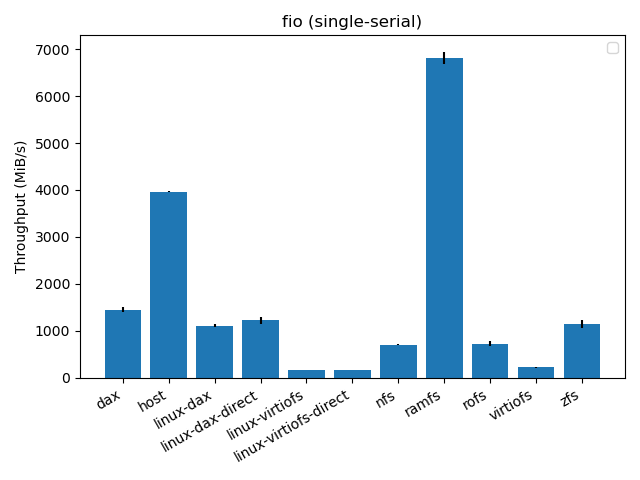
\includegraphics[width=\textwidth]{fio-single-serial-tput}
            \label{fig:fio-single-serial-tput}
        \end{subfigure}
        \begin{subfigure}[c][0.5\textheight]{\textwidth}
            \caption{\en{CPU usage}}
            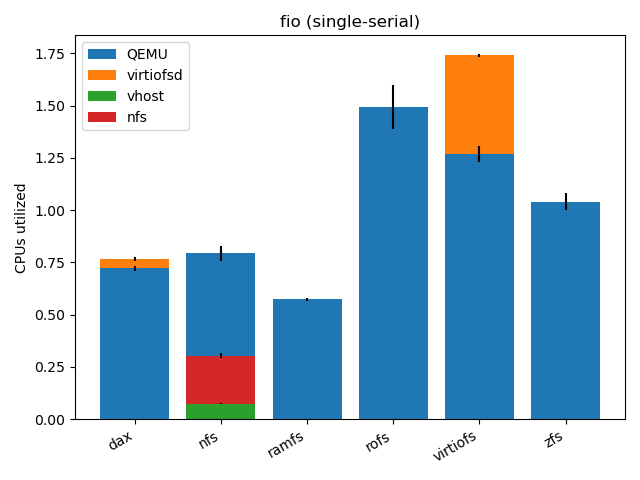
\includegraphics[width=\textwidth]{fio-single-serial-cpu}
            \label{fig:fio-single-serial-cpu}
        \end{subfigure}
        \caption{\en{fio}, ένα αρχείο, σειριακή ανάγνωση}
        \label{fig:fio-single-serial}
    \end{minipage}
\end{figure}

\begin{figure}
    \begin{minipage}[c][\textheight]{\textwidth}
        \begin{subfigure}[c][0.5\textheight]{\textwidth}
            \caption{\en{Throughput}}
            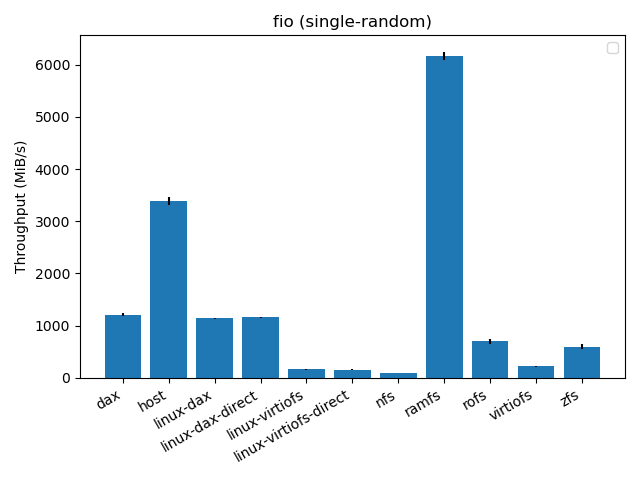
\includegraphics[width=\textwidth]{fio-single-random-tput}
            \label{fig:fio-single-random-tput}
        \end{subfigure}
        \begin{subfigure}[c][0.5\textheight]{\textwidth}
            \caption{\en{CPU usage}}
            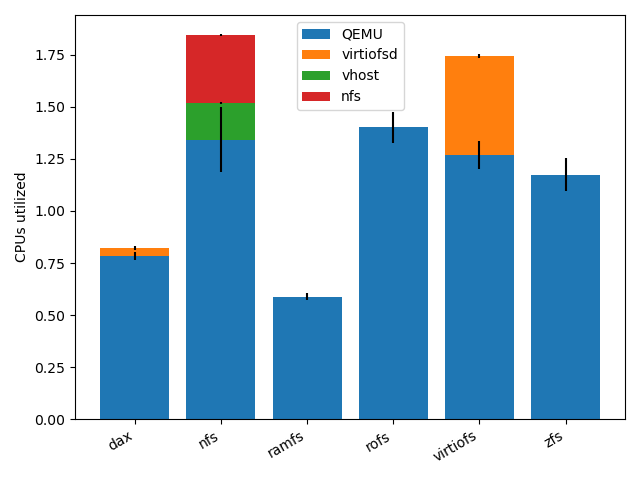
\includegraphics[width=\textwidth]{fio-single-random-cpu}
            \label{fig:fio-single-random-cpu}
        \end{subfigure}
        \caption{\en{fio}, ένα αρχείο, τυχαία ανάγνωση}
        \label{fig:fio-single-random}
    \end{minipage}
\end{figure}

\begin{figure}
    \begin{minipage}[c][\textheight]{\textwidth}
        \begin{subfigure}[c][0.5\textheight]{\textwidth}
            \caption{\en{Throughput}}
            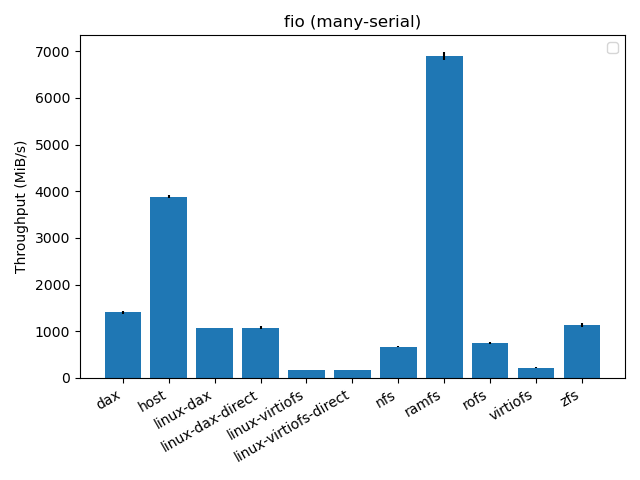
\includegraphics[width=\textwidth]{fio-many-serial-tput}
            \label{fig:fio-many-serial-tput}
        \end{subfigure}
        \begin{subfigure}[c][0.5\textheight]{\textwidth}
            \caption{\en{CPU usage}}
            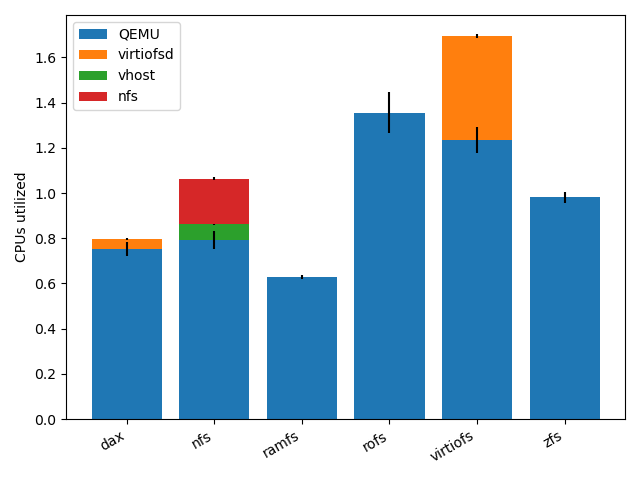
\includegraphics[width=\textwidth]{fio-many-serial-cpu}
            \label{fig:fio-many-serial-cpu}
        \end{subfigure}
        \caption{\en{fio}, πολλαπλά αρχεία, σειριακή ανάγνωση}
        \label{fig:fio-many-serial}
    \end{minipage}
\end{figure}

\begin{figure}
    \begin{minipage}[c][\textheight]{\textwidth}
        \begin{subfigure}[c][0.5\textheight]{\textwidth}
            \caption{\en{Throughput}}
            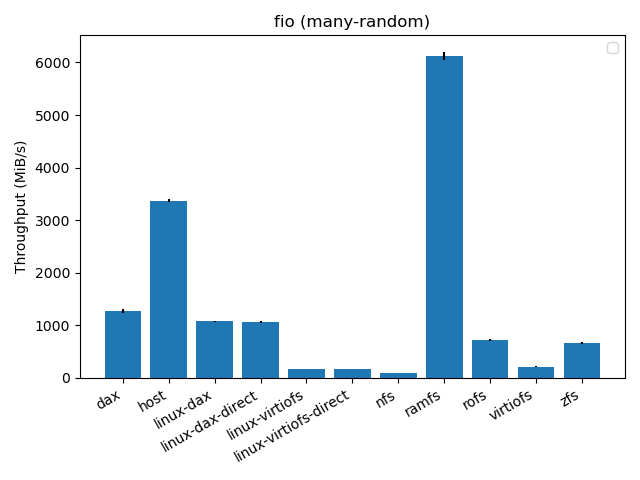
\includegraphics[width=\textwidth]{fio-many-random-tput}
            \label{fig:fio-many-random-tput}
        \end{subfigure}
        \begin{subfigure}[c][0.5\textheight]{\textwidth}
            \caption{\en{CPU usage}}
            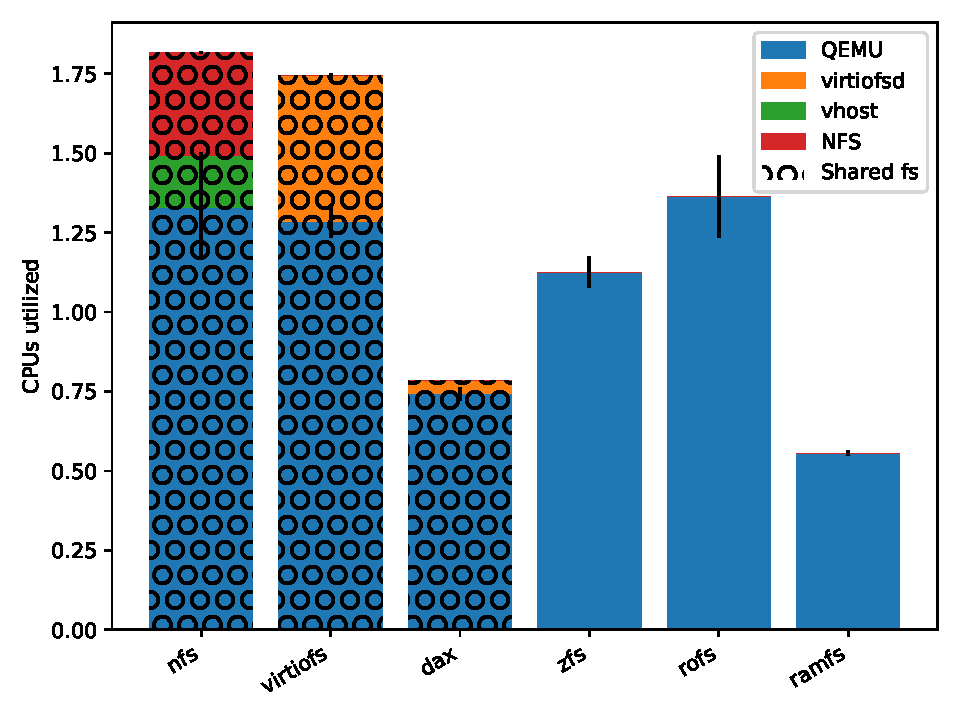
\includegraphics[width=\textwidth]{fio-many-random-cpu}
            \label{fig:fio-many-random-cpu}
        \end{subfigure}
        \caption{\en{fio}, πολλαπλά αρχεία, τυχαία ανάγνωση}
        \label{fig:fio-many-random}
    \end{minipage}
\end{figure}

% tst   OSv    Linux
%  s-s: 220  - 170  (virtio-fs)
%       1450 - 1108 (DAX)
%       707         (NFS)
%  s-r: 217  - 163  (virtio-fs)
%       1212 - 1142 (DAX)
%       85          (NFS)
%  m-s: 219  - 166  (virtio-fs)
%       1402 - 1071 (DAX)
%       668         (NFS)
%  m-r: 215  - 166  (virtio-fs)
%       1269 - 1081 (DAX)
%       85          (NFS)
% mean: 217  - 166  (virtio-fs)
%       1333 - 1100 (DAX)
%       386         (NFS)

Όπως βλέπουμε στα σχήματα \ref{fig:fio-single-serial} έως
\ref{fig:fio-many-random}, το υψηλότερο \en{throughput} επιτυγχάνεται από το
\en{ramfs} στο \osv{}, υψηλότερο και από αυτό του \en{tmpfs} στον \host{}. Αυτό
συμβαίνει διότι, με τα δεδομένα στη μνήμη το \en{virtualization overhead}
ελαχιστοποιείται, ενώ ταυτόχρονα η απλοποιημένη υλοποίηση του συστήματος αρχείων
και η έλλειψη \en{mode switches} λόγω κλήσεων συστήματος στο \osv{} φαίνεται ότι
κάνουν τη διαφορά. Το \viofs{} με \en{DAX} προσφέρει τις αμέσως καλύτερες
επιδόσεις στο \osv{}, σε όλες τις περιπτώσεις, και παράλληλα έχει τη μικρότερη
επιβάρυνση σε όρους επεξεργαστικής ισχύος, και πάλι μετά το \en{ramfs}.

Εστιάζοντας στο \viofs{} και συγκρίνοντας ανάμεσα σε \osv{} και \linux{},
διακρίνουμε συνεπή συμπεριφορά σε όλες τις περιπτώσεις: σε αμφότερα τα
λειτουργικά το \en{DAX window} υπερτερεί του \viofs{} χωρίς αυτό με μεγάλη
διαφορά (\(> 6 \times\) \en{throughput}), ενώ στο \osv{} βλέπουμε \(20 - 30 \%\)
καλύτερες επιδόσεις από ότι στο \linux{}. Το δεύτερο είναι αναμενόμενο, αφενός
λόγω της απλούστερης υλοποίησης στο \osv{}, που υποστηρίζει πολύ λιγότερες
λειτουργίες και αφετέρου λόγω των συγκριτικών πλεονεκτημάτων ενός
\en{unikernel}.

Ιδιαίτερη μνεία οφείλουμε στη σύγκριση ανάμεσα σε \viofs{} και \en{NFS}, τα μόνα
κοινόχρηστα συστήματα αρχείων στο \osv{}. Εδώ το \viofs{} με \en{DAX window}
έχει το προβάδισμα στις επιδόσεις, με το \en{NFS} να ακολουθεί και το \viofs{}
χωρίς \en{DAX} να βρίσκεται τελευταίο, στις δοκιμές με σειριακή ανάγνωση.
Όπως φαίνεται και στον πίνακα \ref{tab:fio-virtiofs-nfs}, στις δοκιμές τυχαίας
ανάγνωσης τα αποτελέσματα διαφοροποιούνται, με το \en{NFS} να έχει το χειρότερο
\en{throughput} (και μεγαλύτερο \en{CPU usage}), έχοντας επηρεαστεί σαφώς
περισσότερο σε σχέση με το \viofs{} από την αλλαγή στο \en{access pattern}.

\begin{table}
    \centering
    \begin{tabular}{ |c|c|c|c| }
        \hline
        \en{pattern} & \viofs{} & \en{NFS} & \viofs{} \en{DAX} \\
        \hline
        σειριακό & 1,0 & 3,1 & 6,5 \\
        τυχαίο & 1,0 & 0,4 & 5,7 \\
        \hline
    \end{tabular}
    \caption{Κανονικοποιημένο \en{fio throughput} \viofs{} και \en{NFS} στο
        \osv{}.}
    \label{tab:fio-virtiofs-nfs}
\end{table}

\section{Χρόνος εκκίνησης}
\subsection{Περιγραφή}
Προκειμένου να αξιολογήσουμε τον χρόνο εκκίνησης στο \viofs{} επιλέξαμε μία
εφαρμογή από αυτές που έχουν ήδη μεταφερθεί στο \osv{} ως παραδείγματα
\cite{osv-apps}. Συγκεκριμένα, επελέγη το \en{spring-boot-example}, μια απλή
\en{web} εφαρμογή από το \cite{spring-boot-examples}
χτισμένη με το \en{spring boot framework}, % ref https://spring.io/projects/spring-boot
στην έκδοση του 2.3.4.%
\footnote{Όλες οι αλλαγές που έγιναν για τις δοκιμές μας βρίσκονται στο
``\en{virtiofs-tests}'' \en{branch} του \en{git repository
\url{https://github.com/foxeng/osv-apps}}.}
Ως \en{Java runtime} επιλέξαμε και πάλι από την ίδια
συλλογή εφαρμογών το \en{openjdk8-zulu-full}. % ref https://github.com/cloudius-systems/osv-apps/tree/master/openjdk8-zulu-full
Η επιλογή της συγκεκριμένης εφαρμογής έγινε καθώς θεωρήθηκε αντιπροσωπευτική,
ως \en{stateless web app}, εφαρμογής που θα γινόταν \en{deploy} ως
\en{unikernel}, σε ένα πλαίσιο \en{cloud}.

Στις δοκιμές συμμετείχαν όλα τα συστήματα αρχείων του \osv{} τα οποία μπορούν να
χρησιμοποιηθούν ως \en{root file systems: ZFS, rofs, ramfs} και \viofs{}.

Η διαδικασία περιελάμβανε την εκκίνηση του \osv{} με το εκάστοτε σύστημα αρχείων
να χρησιμοποιείται ως \en{root file system}. Αυτό αφηνόταν να τρέξει για ένα
εύλογο χρονικό διάστημα κάποιων δευτερολέπτων, μέσα στο οποίο ολοκληρωνόταν η
πλήρης αρχικοποίηση της εφαρμογής και στη συνέχεια τερματιζόταν από το μηχανισμό
(\en{script}) ενορχήστρωσης των δοκιμών, τερματίζοντας τη διεργασία του \qemu{}.

\subsection{Αποτελέσματα}
Στο σχήμα \ref{fig:startup-app} απεικονίζεται μία ανάλυση του συνολικού χρόνου
εκκίνησης ως εξής:
\begin{description}
    \item[\en{OSv boot}] είναι ο χρόνος εκκίνησης (\en{boot}) του συστήματος του
                         \osv{}, δηλαδή του μέρους που είναι ανεξάρτητο της
                         εκάστοτε εφαρμογής.
    \item[\en{Root fs mount}] είναι ο χρόνος προσάρτησης (\en{mount}) του
                              \en{root file system} και της αλλαγής της
                              ``ρίζας'' (\en{/}) του εικονικού συστήματος
                              αρχείων σε αυτό (\en{pivot}). Επισημαίνεται ότι
                              αυτό είναι ένα στάδιο του προηγούμενου, αλλά εν
                              προκειμένω έχει αφαιρεθεί από εκείνο και
                              παρουσιάζεται χωριστά.
    \item[\en{Application}] είναι o χρόνος αρχικοποίησης της ίδιας της
                            εφαρμογής, όπως καταγράφεται από αυτήν.
\end{description}

\begin{figure}
    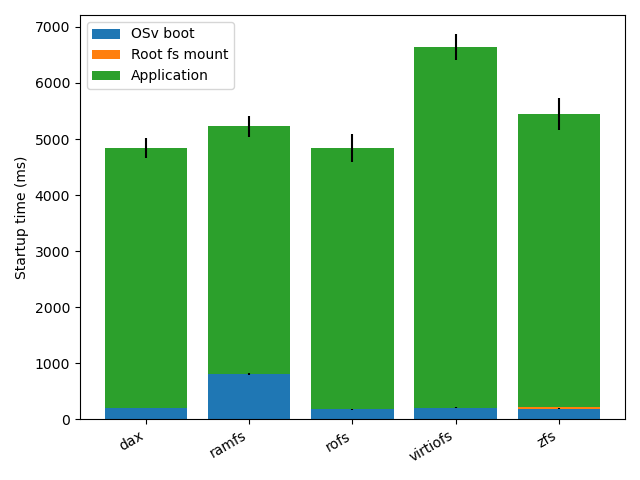
\includegraphics[width=\textwidth]{startup-app}
    \caption{\en{Spring boot example}, χρόνοι εκκίνησης}
    \label{fig:startup-app}
\end{figure}

% fs        total time
% ZFS       5452
% rofs      4838
% ramfs     5226
% virtio-fs 6642
% DAX       4844

Όπως βλέπουμε καλύτερα στον πίνακα \ref{tab:startup-total}, με όρους συνολικού
χρόνου εκκίνησης, το \viofs{} \emph{χωρίς} \en{DAX window} υστερεί έναντι των
υπολοίπων, ενώ το \viofs{} \emph{με} \en{DAX window} έχει την καλύτερη επίδοση,
μαζί με το \en{rofs} (τα \en{ramfs} και \en{ZFS} είναι ελαφρώς πιο αργά).

\begin{table}
    \centering
    \begin{tabular}{ |c|c|c|c|c| }
        \hline
        \en{ZFS} & \en{rofs} & \en{ramfs} & \viofs{} & \viofs{} \en{DAX} \\
        \hline
        1,13 & 1,00 & 1,08 & 1,37 & 1,00 \\
        \hline
    \end{tabular}
    \caption{Κανονικοποιημένος συνολικός χρόνος εκκίνησης
        \en{spring-boot-example} στο \osv{}.}
    \label{tab:startup-total}
\end{table}

Όσον αφορά τον χρόνο προσάρτησης (\en{mount time}), για όλα τα συστήματα αρχείων
είναι πρακτικά αμελητέος (\(<2\%\) του \osv{} \en{boot time}), \emph{εκτός από
το \en{ZFS}}. Στην περίπτωση του τελευταίου, ο χρόνος προσάρτησης αποτελεί
περίπου το \(14\%\) του χρόνου εκκίνησης του συστήματος, κάτι αναμενόμενο
δεδομένης της πολυπλοκότητας του συγκεκριμένου συστήματος αρχείων, η οποία
μεταφράζεται σε μία σαφώς πιο μακρά διαδικασία αρχικοποίησης.

Τέλος, αξίζει να αναφερθούμε στον αισθητά αυξημένο χρόνο εκκίνησης του \osv{}
στην περίπτωση του \en{ramfs}. Αυτή η διαφοροποίηση δικαιολογείται εάν
αναλογιστούμε ότι στην περίπτωση του \en{ramfs}, το \en{root file system}
\emph{ταυτίζεται} με το \en{boot file system} (σε ορολογία \osv{}, το αντίστοιχο
\en{initramfs} στο \linux{}). Αυτό είναι μέρος του \en{ELF object} που περιέχει
το \en{kernel}, το οποίο φορτώνεται και αποσυμπιέζεται κατά τα πρώιμα στάδια του
\en{boot} \cite{osv-wiki}, σε μια διαδικασία με χαμηλό \en{throughput}, λόγω του
περιορισμένου αρχικού περιβάλλοντος. Έτσι, όταν στην περίπτωση του \en{ramfs},
το εν λόγω \en{ELF object} είναι έως και μία τάξη μεγέθους μεγαλύτερο από τα
υπόλοιπα, αυτό είναι υπαίτιο για την αύξηση του χρόνου εκκίνησης. Βέβαια, εν
προκειμένω έχουμε κάνει κατάχρηση του \en{ramfs}, το οποίο δεν είναι προορισμένο
για τόσο μεγάλα \en{images}.

\section{\en{Application benchmark}}
\subsection{Περιγραφή}
Για να αξιολογήσουμε το \viofs{} με όρους μιας ολοκληρωμένης, πραγματικής
εφαρμογής επιλέξαμε και πάλι από το πεδίο των \en{stateless} εφαρμογών σε
πλαίσιο \en{cloud} το σενάριο ενός στατικού \en{web} εξυπηρετητή (\en{server}).
Συγκεκριμένα, χρησιμοποιήσαμε τον \en{nginx} \cite{nginx} (στην έκδοση του
1.19.2), έναν από τους πλέον δημοφιλείς \en{web servers} ελεύθερου λογισμικού, ο
οποίος είναι επίσης διαθέσιμος στη συλλογή εφαρμογών του \osv{}.%
\footnote{Όλες οι αλλαγές που έγιναν για τις δοκιμές μας βρίσκονται στο
``\en{virtiofs-tests}'' \en{branch} του \en{git repository
\url{https://github.com/foxeng/osv-apps}}.}

Στις δοκιμές συμμετείχαν τα όλα τα συστήματα αρχείων του \osv{} (στην περίπτωση
του \viofs{}, ως \en{root file system} χρησιμοποιήθηκε το \en{ramfs})
\emph{εκτός από το \en{NFS}}, με το οποίο το σενάριο μας αποτύγχανε.
Συγκεκριμένα, κατά την εξυπηρέτηση του πρώτου αιτήματος (\en{request}) από τον
\en{server}, μετά την αποστολή λίγων αρχικών δεδομένων της απάντησης
(\en{response}), η διαδικασία σταματούσε και ο \guest{} φαινόταν ``παγωμένος''.
Αυτό διαπιστώθηκε ότι δεν οφείλονταν στον \en{nginx}, καθώς την ίδια ακριβώς
συμπεριφορά επιδείκνυε το σύστημα με τον \en{lighttpd} (επίσης περιλαμβάνεται
στη συλλογή του ``\en{osv-apps}'') στη θέση του. Περαιτέρω διερεύνηση απαιτείται
για να εντοπιστεί και πιθανώς να διορθωθεί η αιτία, η οποία από την εμπειρία μας
φαίνεται να μοιάζει με κάποιου είδους ``αδιέξοδο'' που πιθανώς να εντοπίζεται
στην υλοποίηση του \en{NFS} ή της στοίβας δικτύωσης του \osv{}.

Τα αρχεία τα οποία εξέθετε ο \en{web server} ήταν συνολικά 10, με μέγεθος που
κυμαίνονταν από περίπου 500 \en{KiB} μέχρι και 12 \en{MiB}. Το μέγεθος κάθε
αντίστοιχου αρχείου ήταν σταθερό σε όλες τις δοκιμές.

Για την διεξαγωγή των δοκιμών, που είχαν τη μορφή δοκιμών φορτίου \en{HTTP}
(\en{HTTP load tests}), από τη μεριά του πελάτη (\en{HTTP client})
χρησιμοποιήσαμε το \en{vegeta} \cite{vegeta}, ένα δημοφιλές εργαλείο γι' αυτό το
σκοπό, στην έκδοση του 12.8.3. Η διαδικασία (αυτοματοποιημένη από το \en{script}
ενορχήστρωσης) είχε ως εξής:
\begin{enumerate}
    \item Αρχικά εκκινούνταν ο \osv{} \guest{}, στον οποίο δίνονταν ένα
          δευτερόλεπτο περιθώριο προκειμένου να ολοκληρωθεί η αρχικοποίηση του
          \en{nginx server}).
    \item Στον \host{} εκκινούσε το \en{vegeta}, ρυθμισμένο να παράγει \en{HTTP
          1.1 GET requests} για όλα τα αρχεία του \en{server}, με το μέγιστο
          δυνατό ρυθμό, χρησιμοποιώντας 20 ``εργάτες'' και έως 4 \en{CPUs}, με
          την επαναχρησιμοποίηση (\en{keepalive}) των συνδέσεων \en{TCP}
          ενεργοποιημένη.
    \item Μετά από δέκα δευτερόλεπτα, το \en{vegeta} ολοκλήρωνε το έργο του και
          τερματιζόταν, οπότε και ο αυτοματισμός τερμάτιζε τον \guest{} μέσω
          της διεργασίας του \qemu{}.
\end{enumerate}

\subsection{Αποτελέσματα}

\begin{figure}
    \begin{minipage}[c][\textheight]{\textwidth}
        \begin{subfigure}[c][0.5\textheight]{\textwidth}
            \caption{\en{Requests} ανά δευτερόλεπτο}
            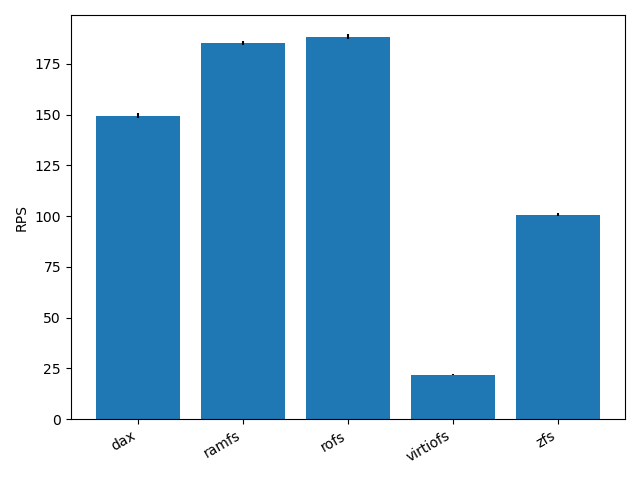
\includegraphics[width=\textwidth]{nginx-rps}
            \label{fig:nginx-rps}
        \end{subfigure}
        \begin{subfigure}[c][0.5\textheight]{\textwidth}
            \caption{\en{CPU usage}}
            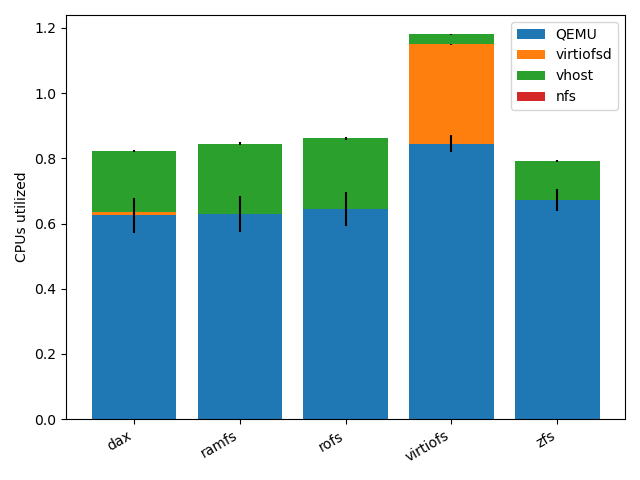
\includegraphics[width=\textwidth]{nginx-cpu}
            \label{fig:nginx-cpu}
        \end{subfigure}
        \caption{\en{nginx HTTP load test}}
        \label{fig:nginx}
    \end{minipage}
\end{figure}

% fs        rps
% ZFS       100
% rofs      188
% ramfs     185
% virtio-fs 150
% DAX       22

Όπως βλέπουμε στο σχήμα \ref{fig:nginx-rps}, το \viofs{} με \en{DAX window}
προσφέρει \en{throughput} (σε όρους εξυπηρετούμενων αιτημάτων ανά δευτερόλεπτο)
που υπολείπεται αυτού των \en{rofs} και \en{ramfs} (τα οποία προηγούνται) κατά
\(\sim 20\%\). Δεδομένου ότι το \en{CPU usage} είναι οριακά χαμηλότερο από των
άλλων δύο, αυτή η διαφορά χρήζει περαιτέρω μελλοντικής διερεύνησης (μέσω
\en{profiling}), με εστίαση στην υλοποίηση του \viofs{} με \en{DAX read
datapath} στο \osv{}, ως κύριο ύποπτο.

Όπως είναι αναμενόμενο σε αυτό το σενάριο χρήσης, το \viofs{} χωρίς \en{DAX}
υστερεί με διαφορά έναντι όλων των υπόλοιπων συστημάτων αρχείων. Αυτό διότι
είναι το μόνο που δεν χρησιμοποιεί οποιασδήποτε μορφής κρυφή μνήμη (\en{cache})
και κάθε λειτουργία ανάγνωσης συνεπάγεται έξοδο και επεξεργασία στον \host{}
(όπως φαίνεται και από το υψηλό \en{CPU usage}), ενώ αυτές οι λειτουργίες είναι
πολύ συχνές, πολλαπλασιάζοντας τις συνέπειες αυτού του \en{overhead}.
